!TeX root = ../main.tex
% Add the above to each chapter to make compiling the PDF easier in some editors.

\chapter{Definitions and Algorithms}\label{chapter:definitions_algorithms}

\section{Convex Hull}

\subsection{Basics}
\label{sec:basics}
First the Convex Hull will be defined. A set $ s \subseteq \mathbb{R}^2 $ is convex if for  every
two points p and q in $s$ it holds that all points on the line segment connecting p and q 
are in $s$ again. This can be expressed, as the fact that the any convex combination of 
p and q has to be in $s$ again. In Isabelle the convex predicate is defined exactly this way:
\begin{lstlisting}
  definition convex :: 'a real_vector set $\Rightarrow$ bool where
  convex s $\longleftrightarrow$ ($\forall$x$\in$s. $\forall$y$\in$s. $\forall$u$\geq$0. $\forall$v$\geq$s. u + v = 1 $\longrightarrow$ u *$_R$ x + v *$_R$ y $\in$ s)
\end{lstlisting}
The convex hull of a set $s$ is the smallest convex set in which $s$ is contained. 
There are several alternative ways in which the convex hull can be defined.
One possible way is to define it as the intersection of all convex sets containing $s$, which 
is also the definition used in Isabelle/HOL. We have already seen the convex predicate, the hull
predicate is defined as the intersection of all sets t that contain s and fulfill the predicate S.
\begin{lstlisting}
    definition hull :: (a' set $\Rightarrow$ bool) $\Rightarrow$ a' set $\Rightarrow$ a' set where
    S hull s = $\bigcap${t. S t $\land$ s $\subseteq$ t}
\end{lstlisting}
Consequently \lstinline|convex hull s| refers to the intersection of all convex sets that 
contain $s$ and therefore the convex hull of the set $s$.
In the two dimensional case for a finite $s \subset \mathbb{R}^2$, the convex hull CH of $s$ 
is a convex polygon and all the corners of this convex polygon are points from S (see figure 1)\cite{de2000computational}. 
As this thesis will focus on the two dimensional case and only give an outlook on the the 
three dimensional case, we will deal with computing the convex hull of $s \in \mathbb{R}^2$ 
in the following and therefore computing a convex polygon as representation of the convex hull of $s$.  
Assuming no three points in $s$ are colinear, then the edges $E \subseteq s^2$  of the polygon 
can be described as exactly those $(p,q) \in s^2$ for which all points in $s$ lie on the left of the vector $\vec{pq}$. 
Notice that the direction of the vector i.e. from p to q is relevant for expressing that a point
lies on the left of the vector $\vec{pq}$.
Of course the symmetric definition of E as those $(p,q) \in s^2$ for which all points in $s$ lie on the right of the line 
$\vec{pq}$ works as well. The only difference is that in the set of directed edges we get, 
every edge now points into the opposite direction. Both definitions make sense, but 
because there is already infrastructure in place for first definition i.e. $(p,q)$  is 
an edge if and only if all points in s are left of $\vec{pq}$, we will use this definition.
But first we need to state the concept of a point $q$ being left of the vector $\vec{pq}$ more
precicsely, especially when there can be three colinear points in $s$.



\vspace{0.5cm}
\begin{center}

\begin{minipage}[t]{0.4\textwidth}
      \centering
      \includestandalone{figures/concave_set}     
      \captionof{figure}{Non-convex set in 2D}
\end{minipage}
\hfill
\begin{minipage}[t]{0.4\textwidth}
  \centering
  \includestandalone{figures/convex_polygon_example}  % Insert standalone picture in the right half
  \captionof{figure}{Convex polygon, which is the convex hull 
    of the set of points $\{P_0, P_1, P_2 , P_3 ,P_4, P_5 , P_6 \}$}      
\end{minipage}
\end{center}
\vspace{0.5cm}

\subsection{Orientation}
Figure 2.2 shows the convex hull of the points $s = \{P_0, P_1, P_2 , P_3 ,P_4, P_5 , P_6 \}$ in the form of a convex polygon.
When using the previous definition, $(P_4,P_5)$, $(P_5,P_6)$ and $(P_4,P_6)$
would be edges of the convex polygon, because it holds that all points in $s$ are left 
of $\vec{P_4 P_5}$, left of $\vec{P_5 P_6}$ and left of $\vec{P_4 P_6}$. 
This is an unintuitive definition which should be avoided. Therefore we define the 
condition for $(p,q)$ to be an edge of the convex hull polygon more precicsely.
$(p,q) \in s^2$ is an edge of the convex hull polygon if and only if all points $r \in s$ 
are either strictly left of the vector $\vec{p q}$ (p, q and r are not colinear) or 
r is contained in the closed segment between $p$ and $q$. The second part can be written
as \lstinline|r $\in$ closed_segment p q| in Isabelle where \lstinline|closed_segment| is
defined as:
% u::real. 0 $\leq$ u $\and$ u $\leq$ 1 
\begin{lstlisting}
  definition closed_segment :: 'a::real_vector $\Rightarrow$ 'a $\Rightarrow$ 'a set
  where closed_segment a b = {(1 - u) *$_R$ a + u *$_R$ b | u::real. 0 $\leq$ u $\land$ u $\leq$ 1 }
\end{lstlisting}
The fact that r lies strictly left 
of $\vec{p q}$ can be expressed differently by stating that ($p$, $q$ , $r$) 
are making a strictly counterclockwise turn. The three points are written as 
a tuple as it is again necessary to state the order of 
$p$, $q$ and $r$ when talking about a counterclockwise turn. In the following a counterclockwise turn will always refer to a strict 
counterclockwise turn. Checking if a point $r$ lies
strictly left of a vector is an operation that is essential for almost all
convex hull algorithms. To check if the points $((x_1,y_1)$ , $(x_2,y_2)$, $(x_3,y_3))$
make a counterclockwise turn, we can look at the sign of the determinant of the 
following matrix.

\[
\text{det} 
\begin{vmatrix}
1 & x_1 & y_1 \\
1 & x_2 & y_2 \\
1 & x_3 & y_3 \\
\end{vmatrix}
= x_1 (y_2 - y_3 ) + x_2 (y_3 - y_1)+ x_3  (y_1 - y_2)
\]
If the determinant is positive, we know that the sequence $(x_1,y_1), (x_2,y_2) , (x_3,y_3)$
makes a counterclockwise turn, if the determinant is zero we know that the three points are colinear 
and if the determinant is negative, we know the the sequence $(x_1,y_1), (x_2,y_2) , (x_3,y_3)$
makes a clockwise turn. %maybe include figure that show points making clockwise, counterclockwise turn
%and being colinear
In Isabelle the function that calculates the above determinant for three 
points is called \lstinline|det3|.
\begin{lstlisting}
  fun det3:: point $\Rightarrow$ point $\Rightarrow$ point $\Rightarrow$ real where 
  det3 (x1, y1) (x2, y2) (x3, y3) =
  x1 * y2 + y1 * x3 + x2 * y3 - y2 * x3 - y1 * x2 - x1 * y3"
\end{lstlisting}
Based on \lstinline|det3| the \lstinline|ccw'| predicate is defined, which expresses that 
three points (p,q,r) make a counterclockwise turn.
\begin{lstlisting}
  definition ccw' p q r $\longleftrightarrow$ 0 < det3 p q r
\end{lstlisting}
Lastly the predicate \lstinline|ccw'_seg p q r| holds if and only if r either lies 
counterclockwise of $\vec{pq}$ or r is contained in the closed segment between p and q.
\begin{lstlisting}
  definition ccw'_seg p q r = ccw' p q r $\lor$ r $\in$ closed_segment p q
\end{lstlisting}


\subsubsection{Intuition}
\label{det3:intuition}
It is not intuitively clear why \lstinline|0 < det3 (x0,y0) (x1,y1) (x2,y2)| ensures a 
counterclockwise orientation. The \lstinline|det3| function can  be interpreted as calculating 
the determinant of the previously described matrix, but the calculations of the \lstinline|det3|
function can also be reformulated.
\begin{lstlisting}
  lemma det_form: "det3 (x0,y0) (x1,y1) (x2,y2)  =  
        (x1 - x0) * (y2 - y0) - (x2 - x0) * (y1 - y0)" 
\end{lstlisting}
Using this definition \lstinline|0 < det3 (x0,y0) (x1,y1) (x2,y2)| means \newline
$(x1 - x0) * (y2 - y0) - (x2 - x0) * (y1 - y0) > 0$,
which can be reformulated to \newline
$(x1 - x0) * (y2 - y0) >  (x2 - x0) * (y1 - y0)$.
Now assuming $y2 \neq y0 \land y1 \neq y0$ and $sign(y2 - y0) = sign (y1 - y0)$, we get
 $(y2 - y0) / (x2 - x0) >   (y1 - y0) / (x1 - x0)$. Therefore the points 
$(x0,y0),(x1,y1),(x2,y2)$ are orientated counterclockwise if the slope of
$\overrightarrow{p_0 p_2}$ is greater than the slope of $\overrightarrow{p_0 p_1}$
with $p_0 = (x0,y0)$,$p_1 = (x1,y1)$ and $p_2 = (x2,y2)$. 
This should make the connection between the \lstinline|det3| function and the geometric
statement $p_2$ lies counterclockwise of $\overrightarrow{p_0 p_1}$ more obvious.
Lastly even if $sign(y2 - y0) \neq sign (y1 - y0)$ is the case 
and $y2 \neq y0 \land y1 \neq y0 $ still holds, we are still comparing the slopes, the $>$ just 
changes to a $<$.


\subsection{Order}
\label{sec:order}
In both algorithms we need to do the following operation. Given an corner $p$ of the convex polygon,
find another corner by searching for a point $q$ such that for all other points 
$r \in s$ either \lstinline|ccw' p q r| or \lstinline|r $\in$ closed_segment p q|
holds. In short, we search for a $q$ that fulfills  
\lstinline|$\forall$ r $\in$ s. ccw'_seg p q r|. 
Intuitively it makes sense that given a finite 
$s \subseteq \mathbb{R}^2$ and a corner of the convex hull polygon, 
we can find a unique next corner. Figuratively speaking, we rotate a line that 
starts in $p$ counterclockwise until we hit a point $q$, which is going to be the next
corner. If we hit several points at the same time, we are just going to take the point 
further away from $p$. Now to translate this into a formal framework, we start with
the previous definition of finding a $q$ that fulfills 
$\forall r \in s.$ \lstinline|(ccw'_seg p)| $q$ $r$. If \lstinline|(ccw'_seg p)| is a total
order on $s$, we know that such a $q$ exists. That's because q is the minimum
respect to the ordering \lstinline|(ccw'_seg p)|. For \lstinline|(ccw'_seg p)| to be a total order
and for later proofs it is necessary that we derive some form of transitivity for the
counterclockwise orientation. For example it should hold that if \lstinline|(ccw'_seg p a b)|
and \lstinline|(ccw'_seg p b c)| holds, then \lstinline|(ccw'_seg p a c)| should hold 
as well. The same implication should hold when using the \lstinline|(ccw'_seg p)| 
ordering instead of \lstinline|(ccw'_seg p)|. Altough straightforward, this kind of transitivity does not always
hold as the following example shows.

\begin{center}
\begin{minipage}{0.5\textwidth}
  \centering
  \includestandalone{figures/transitivity_counterexample}
  \captionof{figure}{}
\end{minipage}
\end{center}

Clearly \lstinline|(ccw' p$_1$ p$_2$ p$_3$)| holds and also 
\lstinline|(ccw' p$_1$ p$_3$ p$_4$)|, but \lstinline|(ccw' p$_1$ p$_2$ p$_4$)| does not hold, instead 
\lstinline|(ccw' p$_1$ p$_4$ p$_2$)| holds. So in order for transitivity to hold, we need to restrict 
the set on which transitivity is supposed to hold. It can be shown that if there exists a $p_0$ such
that for all $r \in s$ it holds that \lstinline|ccw'_seg p$_0$ p$_1$ r| holds, then  
\lstinline|(ccw'_seg p$_1$)| is transitive on $s$. This restriction avoids the counterexample
for general transitivity from above. Transitivity also holds if there exists a point $p_0$ such 
that all $r \in s$ are lexicographically bigger than $p_0$, meaning $\forall r \in s.$ \lstinline|lex p$_0$ r| holds,
where \lstinline|lex| is defined as.
\begin{lstlisting}
  definition lex:: point $\Rightarrow$ point $\Rightarrow$ bool where
  "lex p q $\longleftrightarrow$ (fst p < fst q $\lor$ fst p = fst q $\land$ snd p < snd q $\lor$ p = q)"
\end{lstlisting}
To check if $p$ is lexicographically smaller than $q$, we check if $p_x$ is smaller than $q_x$. If 
they are equal we check if $p_y \leq q_y$ holds. Now given for our reference set 
$ps \subseteq \mathbb{R}^2$ if $(\forall q \in ps.$  \lstinline| ccw'_seg  p_stl p_last q| $)\lor($
$\forall q \in ps.$ \lstinline|lex p_last q| $)$ holds, then the following lemmas can be proven.
\begin{lstlisting}
  lemma ccw'_seg_trans:
  assumes "p $\in$ ps" "q $\in$ ps" "k $\in$ ps"
  assumes "ccw'_seg p_last p q" "ccw'_seg p_last k p"
  shows "ccw'_seg p_last k q"
\end{lstlisting}
\begin{lstlisting}
  lemma ccw'_seg_total:
  assumes "p $\in$ ps" "q $\in$ ps"
  shows "ccw'_seg p_last p q $\lor$ ccw'_seg p_last q p"
\end{lstlisting}
\begin{lstlisting}
  lemma ccw'_seg_antisymmetric:
  assumes "ccw'_seg p_last p q $\land$ ccw'_seg p_last q p"
  shows "p = q"
\end{lstlisting}
Reflexivity directly follows from the definition of \lstinline|ccw'_seg|. Therefore we know
that there exists a unique $q$ such that $\forall r \in ps.$ \lstinline|(ccw'_seg p_last) q r|.
Notice how $ps$ was defined using $p\_last$.
\subsection{Convex Polygon}
\label{sec:conv_poly}
Both algorithms calculate the convex polygon that corresponds to the 
convex hull of the input set $s \subseteq \mathbb{R}^2$. This convex polygon 
is described by a list of points from $s$ that are the corners of this convex polygon.
So far, we just always just stated that the convex polygon corresponds to the 
convex hull, yet it is not obvious that this is the case. Therefore we require a  
description of a convex polygon in Isabelle/HOL and we need 
to know that this description is indeed equivalent to \lstinline|convex hull|, which is defined 
as Intersection of all convex sets that contain $s$. 
To be more precicse, we require a proof that the convex hull of the corners of such a 
convex polygon corresponds to the set of all points that lie within the polygon.
This fact was proven for a list of corners \lstinline|p0 # ps| that should
represent a convex polygon by Simon Hanssen.
\begin{lstlisting}
  lemma polygon_eq_convex_hull:
  assumes turns_only_left (p0 # ps)
      and sorted_wrt (ccw' p0) ps
      and 2 $\leq$ length ps
    shows list_all (encompasses p) (polychain_of (p0 # ps @ [p0]))
       $\longleftrightarrow$ p $\in$ convex hull (set (p0 # ps))"
\end{lstlisting}
To understand this proof, we need to first look at the definitions of all the predicates
used. First \lstinline|turns_only_left l| for a list l expresses that every three consecutive
points in the list are turning counterclockwise. This ensures that every interior angle of 
the polygon is less than $180^\circ$, which is one of the common definitions
of a convex polygon.
\begin{lstlisting}
  fun turns_only_left :: "point list $\Rightarrow$ bool" where
  "turns_only_left (p#q#r#ps) $\longleftrightarrow$ ccw' p q r $\land$ turns_only_left (q#r#ps)"|
  "turns_only_left _ = True"
\end{lstlisting}
Next \lstinline|sorted_wrt (ccw' p0)|, where p0 is the start or our list of corners, states that
for every corner $p$ in the list, all corners that are behind it in the list, lie counterclockwise
of $\overrightarrow{p0  p}$. 
\begin{lstlisting}
  fun sorted_wrt :: "('a $\Rightarrow$ 'a $\Rightarrow$ bool) $\Rightarrow$ 'a list $\Rightarrow$ bool" where
  "sorted_wrt P [] = True" |
  "sorted_wrt P (x # ys) = (($\forall$ y $\in$ set ys. P x y) $\land$ sorted_wrt P ys)"
\end{lstlisting}     
This ensures that the list of corners even represents a polygon
without degenerations like the one shown in Figure \ref{degenerated_corners}. Clearly 
\lstinline|turns_only_left [$p_0$,$p_1$,$p_2$,$p_3$,$p_4$,$p_5$,$p_6$]| holds,
but \lstinline|sorted_wrt (ccw' p0) [ $p_1$,$p_2$,$p_3$,$p_4$,$p_5$,$p_6$]| does not
hold, as the structure in Figure \ref{degenerated_corners} is not a valid polygon.
\begin{center}
  \begin{minipage}{0.5\textwidth}
  \centering
  \includestandalone{figures/degenerated_corner_list}
  \captionof{figure}{}
  \label{degenerated_corners}
\end{minipage}
\end{center}
Lastly \lstinline| 2 $\leq$ length ps | is needed, as the definition does not work in the case 
of two corners, where the polygon is just a closed segment between two points.
Now given a list \lstinline|p0 # ps| fulfills these properties, then we know that this list
describes a list of corners of a convex polygon and the following statement holds.
\begin{lstlisting}
  list_all (encompasses p) (polychain_of (p0 # ps @ [p0]))
       $\longleftrightarrow$ p $\in$ convex hull (set (p0 # ps))
\end{lstlisting}  
Where \lstinline|polychain_of (p0 # ps @ [p0])| is just the list of all tuples of two 
consecutive points in the list and 
\lstinline|encompasses p seg = det3 (fst seg) (snd seg) p $\geq$ 0| states that p lies
counterclockwise (or colinear)  of the vector  $\overrightarrow{(fst \; seg) (snd \; seg)}$. 
With $(fst \; seg)$ being the first point in the tuple  
\lstinline|seg| and $(snd \; seg)$ being the second point in the tuple \lstinline|seg|.
\begin{lstlisting}
  fun polychain_of where
  "polychain_of [] = []"
| "polychain_of [p2] = []"
| "polychain_of (p1#p2#ps) = (p1, p2) # polychain_of (p2 # ps)"
\end{lstlisting}  
The \lstinline|list_all P l| predicate states that the condition \lstinline|P| has to hold
for every element in the list \lstinline|l|.
Consequently \lstinline|list_all (encompasses p) (polychain_of (p0 # ps @ [p0]))| states that p lies
inside the polygon defined by \lstinline|p0 # ps| as it requires that p lies counterclockwise (or colinear) 
of every edge of the polygon. Therefore the lemma \lstinline|polygon_eq_convex_hull| states that a point p
lies inside the convex polygon defined by \lstinline|p0 # ps| if and only if p is in the convex hull
of \lstinline|set (p0 # ps)|. Now we have the definition of a convex polygon and the proof that
the convex hull of the corners of such a 
polygon corresponds to the set of all points that lie within the polygon. Based on this we can show 
that the inspected algorithms, for an input set $s$, compute a convex polygon according to the definition  
and that the convex hull that corresponds to this convex polygon is indeed the convex hull of $s$.




% So given for a list of points  \lstinline|p0 # ps| that contains at least three points, \lstinline|turns_only_left (p0#ps)|
% and \lstinline|sorted_wrt (ccw' p0) ps| holds, then we know that 
% Then we will need to show, that all other points in $s \subseteq \mathbb{R}^2$ (not corners)
% lie inside the convex polygon that is spanned by the corners. 

% Therefore we need a formalization for the convex polygon is and a proof that the
% convex hull of the corners of the polygon is the set of points that lie inside the polygon.  
% From this we will get that both algorithms calculate a list . Then we need to show that all other points in the input set $s$
% lie within this convex polygon and from that we get that the algorithms indeed calculate 
% the convex hull of the input set. In Isabelle/HOL, the 



%might be better to define with {p,q} \in S^2 (i.e. not ordered)



%But the convex hull can also be defined 
%as the set of all convex combinations of points in S, which can be proven equivalent to the previous definition.   


%how is it done in Isabelle
\section{Jarvis-March Algorithm}
\subsection{Definition of the Algorithm}
\label{jarvis:def}
The Jarvis March or Gift-Wrapping Algorithm is a simple output-sensitive way of calculating
the convex hull of a given finite set $S \subseteq \mathbb{R}^2$ of points. It calculates the
convex hull by calculating the corresponding convex polygon and returning
an ordered list of the corners of the polygon. The algorithm has runtime O(n * h), where n 
is the number of points in S and h is the number of points that lie on the convex hull or
the number of corners on the calculated polygon to be more precicse. 
The algorithm starts by choosing a point that is guaranteed to lie on the convex hull. 
We will use the lexicographical minimum $p_0 = \min_{y} \min_{x} S$, or in Isabelle terms
the $p0$, which fulfills \lstinline|$\forall q \in r.$ lex p0 r|.   Then the next corner of the convex polygon
is found by searching a $p_1$ such that every point $r \in s$ lies counterclockwise
of $\vec{p_0 p_1}$ or is contained in the closed segment between $p_0$ and $p_1$, meaning
$\forall r \in ps.$ \lstinline|(ccw'_seg p$_0$) p$_1$ r| should hold. 
As explained in \ref{sec:order} we know  that such a $p_1$ exists, because 
$\forall r \in ps.$ \lstinline|lex p$_0$ r| holds. In Isabelle the definition for
finding the minimum with respect to the total order \lstinline|(ccw'_seg p$_0$)| is.
\begin{lstlisting}
  definition ccw'_seg_min :: " point set $\Rightarrow$ point" where
  "ccw'_seg_min ps =  (THE p. p $\in$ ps $\land$ ($\forall$ q $\in$ ps. ccw'_seg p0 p q))"
\end{lstlisting}  
Now from \ref{sec:basics}, we 
know that $(p_0,p_1)$ is an edge of the wanted convex polygon and 
we know that $p_1$ is once again a point on
the convex hull and a corner of the polygon as $(p_0,p_1)$ fulfills $\forall r \in ps.$ \lstinline|(ccw'_seg p$_0$) p$_1$ r|. 
Therefore we can repeat the previous step
and search for a $p_2$ that fulfills $\forall r \in ps.$ \lstinline|(ccw'_seg p$_1$) p$_2$ r|. 
Once again according to \ref{sec:order}, we know that $\forall r \in ps.$ \lstinline|(ccw'_seg p$_0$) p$_1$ r|
holds and therefore \lstinline|(ccw'_seg p$_1$)| is a total order and a unique $p_2$ exists.
Again $p_2$ has to be a corner of the convex polygon and $(p_1,p_2)$ an edge on of the
polygon. The algorithm continues until a $p_h = p_0$ is found to be the next point and
stops, because the first corner of the polygon is encountered again. 
The ordered sequence of points $p_0,p_q, ... , p_{h-1}$ are the corners of the convex polygon 
and $(p_0,p_1),(p_1,p_2) ... ,(p_{h-2},p_{h-1}), (p_{h-1},p_0)$ are the edges of the polygon.
Figure x shows the steps of Jarvis March computing the convex hull of a input set $ps$.

\newpage
\vspace{0.5cm}

\newpage
% \begin{minipage}{0.4\textwidth}

%   \begin{minipage}[t]{\textwidth}
%     \centering
%     \includestandalone{figures/jarvis_march/input}     
%     \vspace{0.5cm}
%     \captionof{figure}{}
%   \end{minipage}

%   \vspace{1.5cm}

%   \begin{minipage}[t]{\textwidth}
%     \centering
%     \includestandalone{figures/jarvis_march/step1}     
%     \captionof{figure}{}
%   \end{minipage}
%   \vspace{1cm}
%   \begin{minipage}[t]{\textwidth}
%     \centering
%     \includestandalone{figures/jarvis_march/step3}     
%     \captionof{figure}{}
%   \end{minipage}
% \end{minipage}
% % \hfill
% % \vrule width 0.5pt % Vertical line
% % \hfill
% \begin{minipage}{0.4\textwidth}

%   \begin{minipage}[t]{\textwidth}
%     \centering
%     \includestandalone{figures/jarvis_march/lex_min} 
%     \captionof{figure}{}
%   \end{minipage}  

%   \vspace{1.5cm}

%   \begin{minipage}[t]{\textwidth}
%     \centering
%     \includestandalone{figures/jarvis_march/step2} 
%     \captionof{figure}{}      
%   \end{minipage}
%   \vspace{1cm}
%   \begin{minipage}[t]{\textwidth}
%     \centering
%     \includestandalone{figures/jarvis_march/step4} 
%     \captionof{figure}{}      
%     \end{minipage}
% \end{minipage}

% \hfill
% \rule{0.5pt}{\textheight}
% \hfill


\vspace{1cm}

\begin{minipage}[t]{\textwidth}
  \begin{minipage}[t]{0.33\textwidth}
    \centering
    \includestandalone{figures/jarvis_march/input}     
    \captionof{figure}{}
\end{minipage}
\hfill
\begin{minipage}[t]{0.33\textwidth}
  \centering
  \includestandalone{figures/jarvis_march/lex_min}     
  \captionof{figure}{}
\end{minipage}
\end{minipage}
\vspace{1cm}

\begin{minipage}[t]{\textwidth}
  \begin{minipage}[t]{0.33\textwidth}
    \centering
    \includestandalone{figures/jarvis_march/step1}     
    \captionof{figure}{}
\end{minipage}
\hfill
\begin{minipage}[t]{0.33\textwidth}
  \centering
  \includestandalone{figures/jarvis_march/step2}     
  \captionof{figure}{}
\end{minipage}
\end{minipage}
\vspace{1cm}

\begin{minipage}[t]{\textwidth}
  \begin{minipage}[t]{0.33\textwidth}
    \centering
    \includestandalone{figures/jarvis_march/step3}     
    \captionof{figure}{}
\end{minipage}
\hfill
\begin{minipage}[t]{0.33\textwidth}
  \centering
  \includestandalone{figures/jarvis_march/step4}     
  \captionof{figure}{}
\end{minipage}
\end{minipage}

\vspace{1cm}

\begin{minipage}[t]{\textwidth}
  \begin{minipage}[t]{0.33\textwidth}
    \centering
    \includestandalone{figures/jarvis_march/step5}     
    \captionof{figure}{}
\end{minipage}
\hfill
\begin{minipage}[t]{0.33\textwidth}
  \centering
  \includestandalone{figures/jarvis_march/step6}     
  \captionof{figure}{}
\end{minipage}
\end{minipage}


\subsubsection{Jarvis March in Isabelle/HOL}
This repeated finding of the next corner is defined as the function \lstinline|wrap|, where
$q$ is the last minimum that was found and ps is the current set of points we want to find
the convex hull of.
\begin{lstlisting}
function wrap :: "point $\Rightarrow$ point set $\Rightarrow$ point list" where
"wrap q ps =  
(if q = p0 then [] else q#(wrap (ccw'_seg_min q ps) (ps - {q})  ) )"
\end{lstlisting}
The last minimum $q$ is prepended to the list of corners we will return, if we not yet arrived
at the first corner $p0$ again. The next corners are found by  recursively calling \lstinline|wrap|
with the next corner or minimum \lstinline|ccw'_seg_min q ps| and the set $ps - \{q\}$. $q$ can be
removed from the set of points we search for the next corner, as $q$ can not be a corner
of the polygon again.
Lastly the algorithm Javis March is defined by an inital call to wrap, but $p0$ is this time
not removed from the set $ps$ we search for the next corner, because $p0$ is the only corner we
can and must encounter twice.
\begin{lstlisting}
  definition "jarvis_march = to_set (wrap (ccw'_seg_min p0 ps) ps)"
\end{lstlisting}  
The \lstinline|to_set| function just turns the list or corners into the appropriate 
definition of the set of points that lie inside the polygon (see \ref{sec:conv_poly}).  
\begin{lstlisting}
  fun to_set :: "point list $\Rightarrow$ point set" where
"to_set [] = {p0}" |
"to_set [p] = closed_segment p0 p" |
"to_set qs = {p. list_all (encompasses p) (polychain_of (p0#qs@[p0]))}" 
\end{lstlisting}
The special cases of \lstinline|wrap| returning an empty list or an list with only one element
need more explaination. If \lstinline|(wrap (ccw'_seg_min p0 ps) ps) = []|, then we know
\lstinline|ccw'_seg_min p0 ps = p0| has to hold and therefore $\forall r \in ps.$ \lstinline|ccw'_seg p$_0$ p$_0$ r|.
Intuitively it should be clear, that the only point $r$ that fulfills \lstinline|ccw'_seg p$_0$ p$_0$ r| is $p0$ itself
and therefore $ps$ has to only contain $p0$ and the convex hull of a single point is a set containing this
very point. If \lstinline|(wrap (ccw'_seg_min p0 ps) ps) = [p]|, then we know 
$\forall r \in ps.$ \lstinline|ccw'_seg p$_0$ p r| and $\forall r \in ps.$ \lstinline|ccw'_seg p p$_0$ r|.
Again from geometric intuition it should be clear that  $\forall r \in ps.$ \lstinline|r $\in$ closed_segment p0 p|
should hold, as \lstinline|ccw' p$_0$ p r| or \lstinline|ccw' p p$_0$ r| instantly leads to a contradiction.
The last case of the \lstinline|to_set| function just applies the definition for the 
set of points inside inside a convex polygon, as introduced in \ref*{sec:conv_poly}. 
\subsection{Jarvis March is Convex Hull}
\label{jarvis:proofs}
In the following let $ps \subseteq \mathbb{R}^2$ be the finite set of points of which we want to calculate
the convex hull and let $p0 = min_y min_x ps$ be the lexicographical minimum with which we start 
Jarvis March, i.e. our first corner of the convex polygon. In Isabelle terms, we assume 
\lstinline|$\forall$p $\in$  ps. lex p0 p| \space , \space  \lstinline|p0 $\in$ ps| \space  and \space  \lstinline|finite ps|.
First we need to show that the recursive wrap function terminates. 
% would it be better to change to wrap not removing points from the set ?
% would make proof for turns_only_left etc. a lot simpler /
% but showing termination is probably very difficult 
% maybe explain tradeoff
\begin{lstlisting}
  lemma wrap_dom:
  assumes q $\in$ qs $\land$ p0 $\in$ qs
  assumes "qs $\subseteq$ ps"
  assumes "q = p0 $\lor$ ($\forall$q' $\in$ qs. ccw'_seg p_stl q q')"
  shows "wrap_dom (q,qs)"
\end{lstlisting}
This lemma follows from the step by step 
description of \ref*{jarvis:def}. In every step our last minimum $q$ was either equal to $p0$ (in the beginning) 
which fulfills $\forall r \in ps.$ \lstinline|lex p$_0$ r| or our last minimum fulfilled 
$\forall r \in ps.$ \lstinline|ccw'_seg p q r| (found with \lstinline|wrap|) for some $p$.
In both cases \lstinline|(ccw'_seg q)| is a total order and a new minimum $q_{next}$ such that 
$\forall r \in ps.$ \lstinline|ccw'_seg q q_{next} r| holds, exists (see \ref*{sec:order}). So 
\lstinline| ccw'_seg_min q qs| and therefore every recursive call to \lstinline|wrap| is well-defined. 
Additionally the size of the set with which \lstinline|wrap| is recursively called 
decreases in every iteration. Hence the call  \lstinline|(wrap (ccw'_seg_min p0 ps) ps)|
will terminate.
Now we need to show that the list that \lstinline|(wrap (ccw'_seg_min p0 ps) ps)| 
returns represents a correct convex polygon.
\begin{lstlisting}
lemma wrap_sorted:
  shows "sorted_wrt (ccw' p0) (wrap (ccw'_seg_min p0 ps) ps)"

lemma wrap_turns_left:
  shows "turns_only_left (wrap (ccw'_seg_min p0 ps) ps)"
\end{lstlisting}
We will start with the proof of \lstinline|sorted_wrt (ccw' p0) (wrap (ccw'_seg_min p0 ps) ps)|.
To do this, we first show that the inner call \lstinline|wrap (ccw'_seg_min q qs) (qs - {q})|,
where we assume that $\forall r \in  qs.$ \lstinline|ccw'_seg p q r| holds
for the last minimum $q$ and some $p$, produces a list that is \lstinline|sorted_wrt (ccw' p0)|.
\begin{lstlisting}
  lemma wrap_sorted_ind:
  assumes wrap (ccw'_seg_min q qs) (qs - {q}) = ls
  assumes q $\in$ qs  $\land$ p0 $\in$ qs
  assumes qs $\subseteq$ ps
  assumes ($\forall$r $\in$  qs. ccw'_seg p q r) $\land$ (p0 $\neq$ q)
  shows sorted_wrt (ccw' p0) ls
\end{lstlisting}
The proof works by induction over the list ls. In the inductive case, we 
assume \lstinline|ls = a # b # rs| and that the induction hypothesis holds for \lstinline|b # rs|.
Meaning we want to show  \lstinline| sorted_wrt (ccw' p0) a # b # rs| and assume that 
\lstinline| sorted_wrt (ccw' p0) b # rs| already holds additional to the other assumptions like
$q \in qs$ and \lstinline|$\forall$r $\in$  qs. ccw'_seg p q r |.
As the \lstinline|sorted_wrt (ccw' p0)|
predicate only makes sense for list of at least length two, we can assume 
\lstinline|ls = a # b # rs| in the inductive case.
Due to the properties of \lstinline|wrap|, a and b are minima defined by the 
\lstinline|ccw'_seg_min| function, for example \lstinline|a = (ccw'_seg_min q qs)| has 
to hold. From this, one can show that $\forall r \in  (qs - \{a,b\}).$ \lstinline|ccw'_seg a b r|
and $a \neq p0  \land  b \neq p0$  holds. From $a \neq p0  \land  b \neq p0$ and $p0 \in qs$,
we know that $p0 \in (qs - \{a,b\})$ holds and with that \lstinline|ccw'_seg a b p0| has to
hold. But because we assumed $p0$ to be the lexicographical minimum of $ps$ and 
$a \in ps  \land  b \in ps$, we know \lstinline|lex p0 a  $\land$ lex p0 b| has to hold.
From geometric intuition it should be clear, that if \lstinline|lex p0 a  $\land$ lex p0 b|
and $a \neq p0  \land  b \neq p0$, it follows that \lstinline|p0 $\in$ closed_segment a b| can not hold. 
Hence with \lstinline|ccw'_seg a b p0| we know, that \lstinline|ccw' a b p0|
and therefore \lstinline|ccw' p0 a b| has to hold. Using the induction hypothesis 
\lstinline| sorted_wrt (ccw' p0) b # rs|, we know that \lstinline| $\forall r \in$  set rs. ccw' p0 b r|
holds. From $\forall r \in ps.$ \lstinline|lex p$_0$ r|, we know that \lstinline|(ccw' p0)| is 
a total order on $ps$ and therefore also transitive on $ps$. Each element in the list $rs$ is 
indirectly picked from $ps$, which implies \lstinline|(set rs) $\subseteq$ ps|.
So in the end, from \lstinline| $\forall r \in$  set rs. ccw' p0 b r| and \lstinline|ccw' p0 a b|
follows with transitivity \lstinline| $\forall r \in$  set (b#rs). ccw' p0 a r|. Again
together with the induction hypothesis \lstinline| sorted_wrt (ccw' p0) a # b # rs| follows,
which is what we wanted to show.
The final lemma for \lstinline| sorted_wrt (ccw' p0) (wrap (ccw'_seg_min p0 ps) ps) | works
very similar, but a slightly different approach is needed, because in the first step the 
old minimum $p0$  is not removed from $ps$ for the call to \lstinline|wrap|.

Now we want to show the second part \lstinline|turns_only_left (wrap (ccw'_seg_min p0 ps) ps)|.
Again we start with the inner call \lstinline|wrap (ccw'_seg_min q qs) (qs - {q})|.
\begin{lstlisting}
  lemma wrap_turns_left_ind:
  assumes "wrap (ccw'_seg_min q qs)  (qs - {q}) = ls"
  assumes q $\in$ qs  $\land$ p0 $\in$ qs
  assumes qs $\subseteq$ ps
  assumes ($\forall$r $\in$  qs. ccw'_seg p q r) $\land$ (p0 $\neq$ q)
  shows " turns_only_left ls"
\end{lstlisting}
Similar to before in the inductive case, we assume \lstinline|ls = k # q # p # rs|
and can show using the other assumptions and the induction hypothesis that
\lstinline|turns_only_left q # p # rs| already holds. Now we want to show  
\lstinline|turns_only_left k # q # p # rs|, which in this case only requires to
show \lstinline|ccw' k q p|, because of the induction hypothesis. Again the points 
k q and p are defined by \lstinline|ccw'_seg_min| and we can show that    
$\forall r \in  (qs - \{k,q\}).$ \lstinline|ccw'_seg k q r| and \lstinline|ccw'_seg k q p| 
holds. Now if \lstinline|p $\in$ closed_segment k q| would hold, then k, q and p would be
colinear. Also from the previously shown wrap\_sorted\_ind we know, that 
\lstinline|ccw' p0 k q| and \lstinline|ccw' p0 q p| hold. From this and the fact
that k q and p are colinear it would follow that \lstinline|q $\in$ closed_segment k p|,
which should be apparent from an geometric viewpoint. But if 
\lstinline|p $\in$ closed_segment k q| and \lstinline|q $\in$ closed_segment k p| holds,
then it can be shown that $p = q$ has to hold, which is a contradiction to for example 
\lstinline|ccw' p0 q p|. Therefore \lstinline|p $\in$ closed_segment k q| can not hold
and with \lstinline|ccw'_seg k q p|, it follows that \lstinline|ccw' k q p| has to hold,
which shows the lemma.
So \lstinline|(wrap (ccw'_seg_min p0 ps) ps)| does indeed produce a convex polygon. 
Finally we can show the lemma \lstinline|jarvis_eq_convex_hull|.
\begin{lstlisting}
  lemma jarvis_eq_convex_hull:
  "jarvis_march p0 ps = convex hull ps"  
\end{lstlisting}
Applying the definition of the jarvis\_march function, we have to show \\
\lstinline|to_set (wrap (ccw'_seg_min p0 ps) ps) = convex hull ps|.
Why this equality holds if \lstinline|wrap (ccw'_seg_min p0 ps) ps| returns an empty list 
or a list with one element was already explained when the \lstinline|to_set| function
was defined (see \ref*{jarvis:def}). If the list \lstinline|ls = wrap (ccw'_seg_min p0 ps) ps| contains at 
least two points, we know from \lstinline|wrap_sorted| and \lstinline|wrap_turns_left|, that
$ls$ correctly represents a convex polygon. As $ls$ represents a correct convex polygon and 
contains at least two points, we know \lstinline|jarvis_march p0 ps = to_set ls|
is the set of points inside the corresponding polygon. 
\begin{lstlisting}
to_set ls = {p. list_all (encompasses p) polychain_of (p0#ls@[p0])}  
\end{lstlisting}
With \lstinline|wrap_sorted|, \lstinline|wrap_turns_left| and \lstinline|polygon_eq_convex_hull|,
we then know that the set of points inside the polygon is equal to the convex hull of the corners.
\begin{lstlisting}
{p. list_all (encompasses p) polychain_of (p0#ls@[p0])} = convex hull (set p0#ls) 
\end{lstlisting}
This is almost what we wanted to show.
All points in $ls$ are points from $ps$, they are precicsely the points that were identified as
corners of the convex polygon that is the convex hull of $ps$. When we start with 
a call \lstinline|(wrap (ccw'_seg_min p0 ps) ps)| to the wrap function, we know
that in every recursive call to \lstinline|wrap|, one point will be removed from $ps$
until $p0$ is encountered and ls ist returned. The points that are removed from $ps$
throughout the recursion are exactly the points in $ls$. 
With that we also know, that the points \lstinline|ps - (set ls)| are in the set that 
is considered for the next corner in every recursive step of 
\lstinline|(wrap (ccw'_seg_min p0 ps) ps)|. This implies that 
for every $r$ in \lstinline|ps - (set ls)| and every two consecutive corners 
$p$, $q$ in $ls$ it holds that \lstinline|ccw'_seg p q r|. This is because $q$ is found 
as minimum with respect to \lstinline|(ccw'_seg p)| and $r$ has to be in the set 
in which we search the minimum.  Therefore this $r$ 
lies inside the polygon defined by $ls$, as \lstinline|ccw'_seg p q r $\implies$ det3 p q r $\geq$ 0|
and therefore we know that $r$ lies counterclockwise (or colinear) of 
every edge of the polygon. The edges of the polygon are exactly the elements of 
the list \lstinline|polychain_of (p0#ls@[p0])|.  
Meaning we know \lstinline|list_all (encompasses $r$) polychain_of (p0#ls@[p0])|
holds
and the inside of the polygon is
equal to the convex hull of the corners, hence we also know 
\lstinline|r $\in$ convex hull (set p0#ls)|. Finally, we know 
\lstinline|ps - set (ls) $\subseteq$ convex hull (set p0#ls)| and 
\lstinline|set (ls) $\subseteq$ convex hull (set p0#ls)|, which implies \\
\lstinline|convex hull (set p0#ls) = convex hull ps|. Using this equality 
and the previously obtained \lstinline|jarvis_march p0 ps = convex hull (set p0#ls)|, 
we get the final assertion.
\subsection{Computability}
In %\ref{jarvis:proofs}
, the lemma \lstinline|wrap_dom| used, that if we 
call \lstinline|wrap| with a valid last minimum like $p0 = min_y \: min_x \: ps$ in
\lstinline|(wrap (ccw'_seg_min p0 ps) ps)|, then in every 
recursive step with the last minimum being $p \in qs$, \lstinline|(ccw'_seg p)| is a total 
order and transitive on the current set $qs \subseteq ps$. From the fact that \lstinline|(ccw'_seg p)|
is transitive it should be clear, that the minimum can be found by looking at every element 
in $qs$ once, which takes $O(|qs|) \leq O(|ps|) = O(n)$, if n is the number of points in the 
input set for Jarvis March. Comparing two points according to the \lstinline|(ccw'_seg p)|
predicate can be achieved with the following computable function, which can be shown to 
be equivalent to the \lstinline|ccw'_seg| predicate.
\begin{lstlisting}
definition ccw'_seg_fun :: "point $\Rightarrow$ point $\Rightarrow$ point $\Rightarrow$  bool" where
"ccw'_seg_fun p q r = 
(det3 p q r > 0 $\lor$ (det3 p q r = 0 $\land$ dist p r $\leq$ dist p q) )"

lemma ccw'_seg_fun_iff_ccw'_seg:
  assumes  p $\in$ ps $\land$ q $\in$ ps
  shows ccw'_seg_fun p_last p q $\longleftrightarrow$ ccw'_seg p_last p q
\end{lstlisting}
$p$ and $q$ have to be in some $ps$, which fulfills
$\forall r  \in ps.$ \lstinline|ccw'_seg p_stl p_last r| $\lor$ 
$\forall q \in ps.$ \lstinline|lex p_last r| for everything to be well-defined.
Computing the determinant and distance between two points (\lstinline|dist|) only takes
a few arithmetic operations, therefore comparing two points can be seen as an operation 
that takes $O(1)$. 
To sum up, given there are $h$ corners in the convex polygon and $n$ points in the 
input set $ps$, we have to find $h$ times the minimum with respect to a total order
which takes $O(n)$ steps and therefore we get a runtime of $O(h \cdot n)$.
The algorithm is simpler than the Graham Scan or the Chan's algorithm and has a worse
runtime than both unless h is small. Graham Scan achieves a $O(n \cdot log(n))$ runtime and 
Chan's algorithm a $O(n \cdot log(h))$ runtime. If h is small Jarvis March 
can be faster than Graham Scan.

% They were identified by iterating 
% the \lstinline|wrap| function until $p0$ is encountered, where in every iteration, 
% the point \lstinline|l $\in$ ls| that was identified in this iteration is removed from the 
% set with which \lstinline|wrap| continues to iterate. Consequently we know that 
% \lstinline|ps - (set ls)| are never removed from the set over which 
% \lstinline|wrap (ccw'_seg_min p0 ps) ps| iterates, because we start with $ps$ and 
% we never remove any point in \lstinline|ps - (set ls)|. 
% the points that remain in the set over which \lstinline|wrap| iterates until the end.


% As explained in \ref{sec:conv_poly} with the \lstinline|poylgon_eq_convex_hull| lemma
% the proof that Jarvis March calculates the convex hull is almost done. 
% But one problem remains, for the points which    



\section{Graham Scan}
In Simon Hanssen's Bachelor Thesis, it was already shown that the Graham Scan Algorithm
calculates the convex hull of a input set of points. 
However the Graham Scan Algorithm works by first sorting the points and then 
calculating the convex hull. So far it was only shown that given a list of
sorted points $ps$, the second phase of the algorithm correctly calculates
the convex hull. Assuming the points of which we want to calculate
the convex hull are given as a list $ps$ and $p0 = min_y min_x$ \lstinline|(set ps)| is the 
lexicographical minimum, then the proof assumes \lstinline|sorted_wrt (ccw' p0) ps|. 
Therefore we want to implement the sorting phase and show that it produces a list $ps$,
which is \lstinline|sorted_wrt (ccw' p0) ps|. To avoid duplication, an existing framework
for sorting elements according to an order should be used. The Comparator theory provides
a definition for comparing two elements of an arbitrary type.
\begin{lstlisting}
locale comparator =
  fixes cmp :: "'a $\Rightarrow$ 'a $\Rightarrow$ comp"
  assumes refl: "$\forall$ a. cmp a a = Equiv"
      and trans_equiv: "$\forall$ a b c. cmp a b = Equiv $\Longrightarrow$ 
                        cmp b c = Equiv $\Longrightarrow$ cmp a c = Equiv"
  assumes trans_less: "cmp a b = Less $\Longrightarrow$ cmp b c = Less $\Longrightarrow$ cmp a c = Less"
      and greater_iff_sym_less: "$\forall$ b a. cmp b a = Greater $\longleftrightarrow$ cmp a b = Less"

datatype comp = Less | Equiv | Greater

\end{lstlisting} 
The operation \lstinline|cmp| that compares two values of type \lstinline|'a| is defined
to be of the type \lstinline|'a comparator|.
\begin{lstlisting}
  typedef 'a comparator = "{cmp :: 'a $\Rightarrow$ 'a $\Rightarrow$ comp. comparator cmp}"
\end{lstlisting}
Lastly \lstinline|sort| is the already implemented sorting that uses a Comparator,
takes in an arbitrary list and produce a \lstinline|sorted| list.
\begin{lstlisting}
  definition sort :: "'a comparator $\Rightarrow$ 'a list $\Rightarrow$ 'a list"

  lemma sorted_sort :
  "sorted cmp (sort cmp xs)"
\end{lstlisting}
The Comparator framework uses the \lstinline|sorted| predicate to express that a list is 
sorted, therefore we need to translate from the \lstinline|sorted| predicate to
the \lstinline|sorted_wrt| predicate.
\begin{lstlisting}
  lemma sorted_wrt_if_sorted: "sorted cmp ls $\Rightarrow$ 
  sorted_wrt ($\lambda$ a b.(compare cmp a b = Equiv) $\lor$ (compare cmp a b = Less)) ls" 
\end{lstlisting}
The \lstinline|compare| function just applies a Comparator $cmp$ to two elements $a$ and $b$. 
From the fact that the order \lstinline|(ccw' p0)| is in general not transitive (see \ref*{sec:order}),
it should become clear that an intuitive definition like \lstinline|ccw'_comparator| will not work.
\begin{lstlisting}
  lift_definition ccw'_comparator :: "point comparator" 
    is "$\lambda$ p q. if ccw' p0 p q then Less else if ccw' p0 q p then Greater 
                       else Equiv"
\end{lstlisting}
For arbitrary $p$, $q$ and $r$, \lstinline|ccw' p0 p q $\land$ ccw' p0 q r $\implies$ ccw' p0 p r|
does not always hold. If, for example \lstinline|lex p|, \lstinline|lex q| and \lstinline|lex r| is the case,
then the implication does hold. A possible solution to this problem uses a different viewpoint on 
what \lstinline|sorted_wrt (ccw' p0) ps| actually means. Instead of interpreting $ps$ as being sorted
according to \lstinline|(ccw' p0)|, we can interpret $ps$ as being sorted with respect to the angle 
the points in $ps$ form with the x-axis, that goes through $p0$.

\noindent
\begin{minipage}{0.45\textwidth}
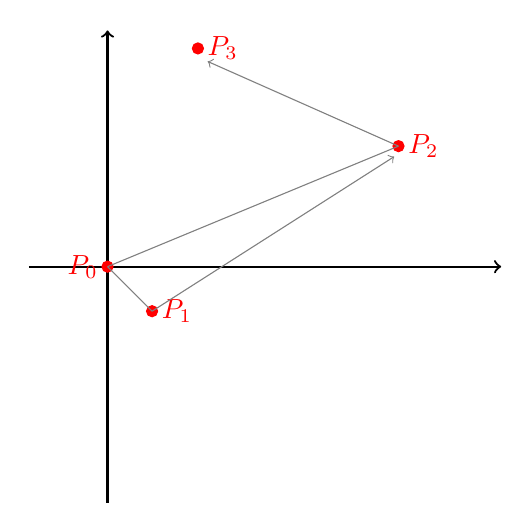
\begin{tikzpicture}

  \draw[->, thick] (-1, 0) -- (5, 0);
  \draw[->, thick] (0, -3) -- (0, 3);
  
  \filldraw[red] (0, 0) coordinate(p0) circle (2pt)  node[left] {$P_0$};
  \filldraw[red] (xyz polar cs:angle=-45,radius=0.8) coordinate(p1) circle (2pt) node[right] {$P_1$};
  \filldraw[red] (xyz polar cs:angle=22.5,radius=4) coordinate(p2) circle (2pt)  node[right] {$P_2$};
  \filldraw[red] (xyz polar cs:angle=67.5,radius=3) coordinate(p3) circle (2pt)  node[right] {$P_3$};
  
  \draw[->,  gray] (p1) -- (xyz polar cs:angle=21,radius=3.9);
  \draw[->,  gray] (p2) -- (xyz polar cs:angle=64,radius=2.9);
  
  \draw[gray] (0,0) -- (p1);
  \draw[gray] (0,0) -- (p2);
  
\end{tikzpicture}
\end{minipage}%
\hfill
\begin{minipage}{0.45\textwidth}
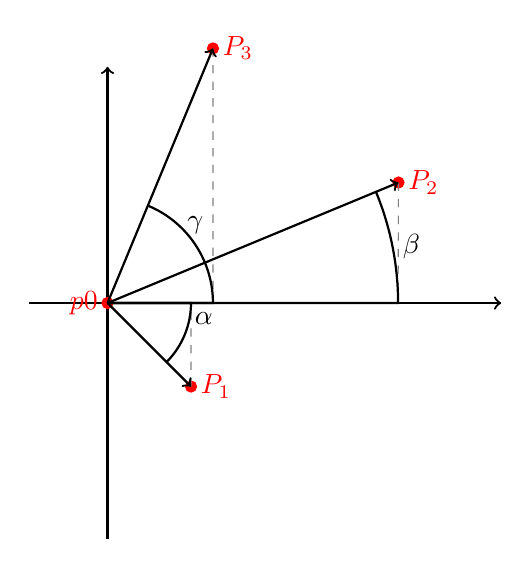
\begin{tikzpicture}

  \draw[->, thick] (-1, 0) -- (5, 0);
  \draw[->, thick] (0, -3) -- (0, 3);
  
  \filldraw[red] (0, 0) coordinate(p0) circle (2pt)  node[left] {$p0$};
  \filldraw[red] (xyz polar cs:angle=-45,radius=1.5) coordinate(p1) circle (2pt) node[right] {$P_1$};
  \filldraw[red] (xyz polar cs:angle=22.5,radius=4) coordinate(p2) circle (2pt)  node[right] {$P_2$};
  \filldraw[red] (xyz polar cs:angle=67.5,radius=3.5) coordinate(p3) circle (2pt)  node[right] {$P_3$};
  
  \draw[gray,dashed] (p1) -- (1.060, 0);
  \draw[gray,dashed] (p2) -- (3.69,0);
  \draw[gray,dashed] (p3) -- (1.339,0);

  % % arking angles and labeling them
  \draw[thick, ->] (0, 0)  -- (p1) {};
  \draw[thick, ->] (0, 0) -- (p2) {};
  \draw[thick, ->] (0, 0) -- (p3) {};
  
  % Drawing arcs for the angles
  \draw[thick] (0,0) -- (1.060, 0) arc[start angle=0, end angle=-45, radius=1.060cm] node[midway, anchor=south west] {$\alpha$};
  \draw[thick] (0,0) -- (3.69, 0) arc[start angle=0, end angle=22.5, radius=3.69cm] node[midway, anchor=west] {$\beta$};
  \draw[thick] (0,0) -- (1.339, 0) arc[start angle=0, end angle=67.5, radius=1.339cm] node[midway, anchor=south] {$\gamma$};

\end{tikzpicture}
\end{minipage}


In Figure x, you can see the lexicographical minimum p0 and a list of points \lstinline|ps = [$P_1$,$P_2$,$P_3$]|
in a coordinate system. Notice that p0 is the lexicographical minimum \lstinline| $p0 = min_y \space min_x$ (set ps $\cup$ {p0}) |, 
where we first minimize x and then y, therefore all points in $ps$ have greater or equal x-values than $p0$ and 
only if they have the same x-value as $p0$, their y-value is greater or equal than the y-value of $p0$.
Clearly the list \lstinline|ps = [$P_1$,$P_2$,$P_3$]| fulfills 
\lstinline|sorted_wrt (ccw' p0) ps|, as \lstinline|ccw' p0 P_1 P_2| and  \lstinline|ccw' p0 P_2 P_3|
holds. But $ps$ is also sorted with respect to the angles that the points form with $x'$, the line parallel
to the x-axis, that goes through $p0$, as $\alpha = -\frac{\pi}{4}$, $\beta = \frac{\pi}{8}$, $\gamma = \frac{3 \pi}{8}$
and $\alpha \le  \beta \le \gamma $ holds. It would also be possible to take the angles, that 
the points form with $y'$ , the line parallel to the y-axis that goes through $p0$. In this case,
we would have angles from $0$ to $\pi$, instead of angles from $-\frac{\pi}{2}$ to  $\frac{\pi}{2}$.
For our purpose taking the angles with respect to $x'$ will be simpler. In the following, we are first
going to calculate the angles, that the points in $ps$ form with $x'$, then we are going to sort the points
in ascending order according to their angles and lastly we have to show that this order is always 
going to be the same as if they were ordered accoring to \lstinline|(ccw' p0)|. The function \lstinline|angle|
calculates the angle formed with $x'$, where $p0 = (x0,y0)$ and $(x1,y1)$ is going to be
a point in $ps$. To be more precicse, the function calculates the angle 
$\mathrel{\text{\large$\angle$}} (x1,y1) (x0,y0) (x0,y1)$ .
\begin{lstlisting}
  fun calc_angle1 :: "point $\Rightarrow$ point $\Rightarrow$ real" where
  "calc_angle1 (x0,y0) (x1,y1) = (if x1 = x0 $\land$ y1 = y0 then -pi/2 else 
                    if x1 = x0 then pi/2 else  arctan ((y1 - y0)/(x1 - x0))) "
\end{lstlisting}
Arcussinus or Arcuscosinus could be used to calculate the angles as well, but we choose 
Arcustanges, as it translates to the \lstinline|(ccw' p0)| ordering more easily.
Essentially we are calculating the Arcustanges of the slope of the vector $\overrightarrow{(x0,y0)(x1,y1)}$.
However the case $x1=x0$ would be undefined, as $(x1 - x0) = 0$, therefore we have to handle this case differently.  
As already explained, if a point $p1$ has the same x-value as $p0$, we know that the y-value of $p1$ has to
be greater or equal than the y-value of $p0$. Therefore, assuming \lstinline|lex p0 p1|, we know that $y1 \ge y0$
has to hold, if $x1 = x0$. Therefore it makes sense to assign the angle $\frac{\pi}{2}$, if $x1 = x0$ 
and \lstinline|lex p0 p1|, which implies $y1 \ge y0$, holds. The case where $x1 = x0 \land y1 = y0$ will be explained 
later. Now we can proof that if two points $p1$ and $p2$ have the same angle with respect
to $p0$ , then $p0$, $p1$ and $p2$ are
colinear.
\begin{lstlisting}
  lemma angle_to_det0:
  assumes  "calc_angle1 (x0,y0) (x1,y1) = calc_angle1 (x0,y0) (x2,y2)" 
  assumes  "x1 $\le$ x0 $\land$ x2 $\le$ x0"
  shows   " det3 (x0,y0) (x1,y1) (x2,y2) = 0" 
\end{lstlisting}
The only interesting case is that $x1 \neq x0 \land x2 \neq x0$ and \\
\lstinline|calc_angle1 (x0,y0) (x1,y1) = calc_angle1 (x0,y0) (x2,y2)| holds, because \\
\lstinline|arctan ((y1 - y0)/(x1 - x0)) = arctan ((y2 - y0)/(x2 - x0))| holds. Then because
of the injectivity of Arcustanges, we know  $\frac{y1 - y0}{x1 - x0} = \frac{y2 - y0}{x2 - x0}$ holds.
From this we get $(y1 - y0) \cdot (x2 - x0) = (y2 - y0) \cdot (x1 - x0)$ and using the \lstinline|det_form|
lemma from \ref{det3:intuition}, we get \lstinline|det3 (x0,y0) (x1,y1) (x2,y2) = 0|. \\
Next we show the central lemma stating that if $(x2,y2)$ forms a greater angle with $x'$ than $(x1,y1)$
does, we know that $(x0,y0)$, $(x1,y1)$, $(x2,y2)$ are oriented counterclockwise.
\begin{lstlisting}
  lemma angle_to_det:
  assumes "calc_angle1 (x0,y0) (x1,y1) $<$ calc_angle1 (x0,y0) (x2,y2)" 
  assumes "lex (x0,y0) (x1,y1)  $\land$ lex (x0,y0) (x2,y2) $\land$ 
            (x0,y0) $\neq$ (x1,y1) $\land$ (x0,y0) $\neq$ (x2,y2)"
  shows   " det3 (x0,y0) (x1,y1) (x2,y2) $>$ 0" 
\end{lstlisting}
Again for now we ignore the case where both arguments of \lstinline|angle| are 
the same point and \lstinline|angle| would evaluate to $-\frac{\pi}{2}$. Then 
the only interesting case is where $x1 \neq x0 \land x2 \neq x0$ holds and 
\lstinline|angle| on both sides evaluates to \lstinline|arctan|, meaning 
\lstinline|arctan ((y1-y0)/(x1-x0)) $<$ arctan ((y2-y0)/(x2-x0))| holds. Then due to 
Arcustanges being strictly monotonically increasing, we know $\frac{y1 -y0}{x1 - x0} < \frac{y2-y0}{x2-x0}$.
From $x1 \neq x0 \land x2 \neq x0$, we know that both sides are well-defined and 
from \lstinline|lex (x0,y0) (x1,y1)| $\land$  \lstinline|lex (x0,y0) (x2,y2)|, we know $x1 \geq x0$
and $x2 \geq x0$ holds. Therefore, we can reformulate $\frac{y1 -y0}{x1 - x0} < \frac{y2-y0}{x2-x0}$
to $(y1 - y0) \cdot (x2 - x0) < (y2 - y0) \cdot (x1 - x0)$, which again using the \lstinline|det_form|
lemma from \ref{det3:intuition} implies that \lstinline|det3 (x0,y0) (x1,y1) (x2,y2) $>$ 0| holds.

Using the \lstinline|arctan| function in \lstinline|angle| is not necessary, it would be fine
to just directly map a point $p$ to the slope of $\overrightarrow{p0 \; p}$ instead of 
\lstinline|arctan| of the slope. Using \lstinline|arctan| and comparing angles
instead of slopes is still preferable, as then \lstinline|angle| is a bounded function. If we would work 
with slopes directly, a case where $x1 = x0$ would have to be mapped to $\infty$ or a 
different special value and a different datatype than \lstinline|real| might be necessary. Comparing
angles is easier for proofs and \lstinline|arctan| guarantees useful properties like boundedness.

\subsection{Colinearity}
\label{graham:colinear}
So far, we ignored a non-trivial problem. The lemma which shows that the Graham Scan 
algorithm calculates the convex hull assumes that the sorting phase produced a list 
$ps$, which is \lstinline|sorted_wrt (ccw' p0) ps|. Therefore $ps$ cannot contain any
$p,q \in$ \lstinline|(set ps)| with $p \neq q$ such that $p0$, $p$ and $q$ are colinear.
Now we cannot assume this for an arbitrary input list or set of points. Therefore we will
show that our implementation of the sorting phase produces a list $ps$ that is 
\lstinline|sorted_wrt (ccw'_seg_rev p0) ps|, where \lstinline|ccw'_seg_rev| is 
defined similar to \lstinline|ccw'_seg|.
\begin{lstlisting}
  definition "ccw'_seg_rev p q r = ccw' p q r $\lor$ q $\in$ closed_segment p r"
\end{lstlisting}
The fact that \lstinline|sorted_wrt (ccw'_seg_rev) ps| holds, is just the formal way 
of expressing that if two points $p$, $q$ cannot be ordered according to \lstinline|(ccw' p0)|, because
neither \lstinline|ccw' p0 p q| nor \lstinline|ccw' p0 q p| holds, they are ordered according to 
\lstinline|(dist p0)|. Therefore if \lstinline|dist p0 p $\leq$ dist p0 q|, then p will preced q in the 
list $ps$. Again this is very similar to \lstinline|ccw'_seg|, just that q would preced p if 
\lstinline|dist p0 p $\leq$ dist p0 q| holds and $ps$ is sorted according to \lstinline|ccw'_seg|.
%maybe show transitivity
As we cannot ensure that the second phase of Graham Scan gets a $ps$ with 
\lstinline|sorted_wrt (ccw' p0) ps|, we want the sorting phase to produce a $ps$, which 
is sorted according to a weaker relation that still ensures that the second phase correctly
computes the convex hull. For Graham Scan to still produce a 
correct convex hull, \lstinline|ccw'_seg_rev| should be used. 

\subsection{Angle Comparator}
We have already 
seen from \lstinline|angle_to_det| and \lstinline|angle_to_det0| that comparing the angles of points
with \lstinline|angle| translates to comparing points with \lstinline|ccw'|.
Now we want to get a comparator \lstinline|angle_comparator|, such that the already implemented 
\lstinline|sort| according to this 
comparator produces a $ps$ that fulfills \lstinline|sorted_wrt (ccw'_seg_rev p0) ps|.
\begin{lstlisting}
  lemma ccw'_seg_rev_if_sorted_w_angle_comp:
  shows "sorted_wrt (ccw'_seg_rev p0) (sort angle_comparator ps)"
\end{lstlisting}
This lemma essentially uses three lemmas. First we use the previously explained \lstinline|sorted_wrt_if_sorted| lemma
to translate from \lstinline|sorted| to \lstinline|sorted_wrt|. Second we need to prove the \lstinline|weaker_rel|
lemma for our specific \lstinline|angle_comparator| and use the \lstinline|sorted_wrt_mono_rel| lemma to 
translate from the \lstinline|angle_comparator| to the \lstinline|(ccw'_seg_rev p0)| predicate.
\begin{lstlisting}
  lemma  weaker_rel:
  assumes ins: "x $\in$ set ps $\land$ y $\in$ set ps"
  assumes rel: "(compare angle_comparator x y = Equiv) 
  $\lor$(compare angle_comparator x y = Less)"
  shows  "ccw'_seg_rev p0 x y"

  lemma sorted_wrt_mono_rel:
  "($\bigwedge$x y. $\llbracket$ x $\in$ set xs; y $\in$ set xs; P x y $\rrbracket$ $\Longrightarrow$ Q x y) 
  $\Longrightarrow$ sorted_wrt P xs $\Longrightarrow$ sorted_wrt Q xs"
\end{lstlisting} 
A first definition of the  \lstinline|angle_comparator| could look like this.
\begin{lstlisting}
  lift_definition angle_comparator :: "point comparator"
  is "$\lambda$ x y. if angle p0 x < angle p0 y then Less 
                else if angle p0 x > angle p0 y then Greater else Equiv"
\end{lstlisting} 
But we also need to deal with the \lstinline|angle p0 x = angle p0 y| case in more
detail, we cannot declare these points as \lstinline|Equiv|. As we have seen before, \lstinline|angle p0 x = angle p0 y| 
implies that $p0$, $p1$ and $p2$ are colinear
and as explained in \ref*{graham:colinear}, we want to compare the distance to p0 
in this case. Therefore the final \lstinline|angle_comparator| will look like this.
\begin{lstlisting}
  definition "angle_comparator = 
  key ($\lambda$p.(calc_angle1 p0 p ,dist p0 p)) lex_comparator"
\end{lstlisting}
\lstinline|key f cmp| creates a comparator, that works as follows.
The new Comparator will first apply f to the two elements to compare and
then compare them with the Comparator cmp. 
\begin{lstlisting}
  lift_definition key :: "('b $\Rightarrow$ 'a) $\Rightarrow$ 'a comparator $\Rightarrow$ 'b comparator"
\end{lstlisting}
The \lstinline|lex_comparator| translates the \lstinline|lex| predicate into a comparator in the 
obvious way. Therefore the \lstinline|angle_comparator| takes two points $p$, $q$ and first maps them to 
tuples \lstinline|(angle p0 p,dist p0 p)|,\lstinline|(angle p0 q,dist p0 q)| and then compares 
themlexicographically, meaning first the angles are compared and if they are the same, the distance to p0
is compared and if the distances are the same, the points are declared as equivalent. Now with this definition
of \lstinline|angle_coomparator| it is possible to show the \lstinline|weaker_rel| lemma and with that the final 
lemma \lstinline|ccw'_seg_rev_if_sorted_w_angle_comp| can be shown.


\section{Chans Algorithm}

Citation test~\parencite{latex}.

Acronyms must be added in \texttt{main.tex} and are referenced using macros. The first occurrence is automatically replaced with the long version of the acronym, while all subsequent usages use the abbreviation.

E.g. \texttt{\textbackslash ac\{TUM\}, \textbackslash ac\{TUM\}} $\Rightarrow$ \ac{TUM}, \ac{TUM}

For more details, see the documentation of the \texttt{acronym} package\footnote{\url{https://ctan.org/pkg/acronym}}.
\subsection{Subsection}

See~\autoref{tab:sample}, \autoref{fig:sample-drawing}, \autoref{fig:sample-plot}, \autoref{fig:sample-listing}.

\begin{table}[htpb]
  \caption[Example table]{An example for a simple table.}\label{tab:sample}
  \centering
  \begin{tabular}{l l l l}
    \toprule
      A & B & C & D \\
    \midrule
      1 & 2 & 1 & 2 \\
      2 & 3 & 2 & 3 \\
    \bottomrule
  \end{tabular}
\end{table}

\begin{figure}[htpb]
  \centering
  % This should probably go into a file in figures/
  \begin{tikzpicture}[node distance=3cm]
    \node (R0) {$R_1$};
    \node (R1) [right of=R0] {$R_2$};
    \node (R2) [below of=R1] {$R_4$};
    \node (R3) [below of=R0] {$R_3$};
    \node (R4) [right of=R1] {$R_5$};

    \path[every node]
      (R0) edge (R1)
      (R0) edge (R3)
      (R3) edge (R2)
      (R2) edge (R1)
      (R1) edge (R4);
  \end{tikzpicture}
  \caption[Example drawing]{An example for a simple drawing.}\label{fig:sample-drawing}
\end{figure}

\begin{figure}[htpb]
  \centering

  \pgfplotstableset{col sep=&, row sep=\\}
  % This should probably go into a file in data/
  \pgfplotstableread{
    a & b    \\
    1 & 1000 \\
    2 & 1500 \\
    3 & 1600 \\
  }\exampleA
  \pgfplotstableread{
    a & b    \\
    1 & 1200 \\
    2 & 800 \\
    3 & 1400 \\
  }\exampleB
  % This should probably go into a file in figures/
  \begin{tikzpicture}
    \begin{axis}[
        ymin=0,
        legend style={legend pos=south east},
        grid,
        thick,
        ylabel=Y,
        xlabel=X
      ]
      \addplot table[x=a, y=b]{\exampleA};
      \addlegendentry{Example A}
      \addplot table[x=a, y=b]{\exampleB};
      \addlegendentry{Example B}
    \end{axis}
  \end{tikzpicture}
  \caption[Example plot]{An example for a simple plot.}\label{fig:sample-plot}
\end{figure}
